\documentclass[crop,tikz]{standalone}
\usetikzlibrary{backgrounds}
\colorlet{blue}{cyan}
\tikzset{
  inverted/.style = {
    color=white,
    background rectangle/.style={fill},
    show background rectangle
  }
}

\usepackage{pgfplots}
\tikzset{>=latex}

\begin{document}
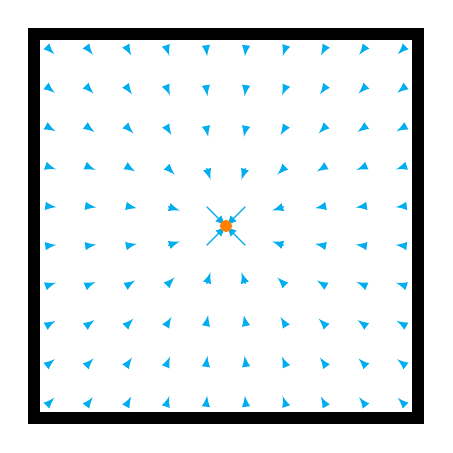
\begin{tikzpicture}[inverted,inverted]
  \begin{axis}[inverted,
    xmin = -2, xmax = 2,
    ymin = -2, ymax = 2,
    axis equal image,
    xtick = {\empty},
    xticklabels = {\empty},
    ytick = {\empty},
    yticklabels = {\empty},
    view = {0}{90},
    height=6cm,
    samples = 10,
    color = blue,
    domain = -2:2,
    hide axis,
    clip = false,
    ]
    \addplot3[
      point meta = {pow(x^2+y^2,-0.1)},
      quiver = {
        u = {-x/(x^2+y^2)},
        v = {-y/(x^2+y^2)},
        scale arrows = 0.1,
        every arrow/.append style={%
           -{latex[scale={max(0.7,\pgfplotspointmetatransformed/1000)}]},
        },
      },
      ->,
    ] {0};
    \draw[fill,orange] (axis cs: 0,0) circle[radius=2pt] node[below=0.5em,white] {$q_1$};
  \end{axis}
\end{tikzpicture}
\end{document}
